\documentclass[tikz,border=10pt,varwidth=200cm]{standalone}
\usepackage[utf8]{inputenc}
\usepackage[T1]{fontenc}
\usepackage{xcolor}
\usepackage{tikz}
\usetikzlibrary{shapes, arrows, positioning}
\begin{document}
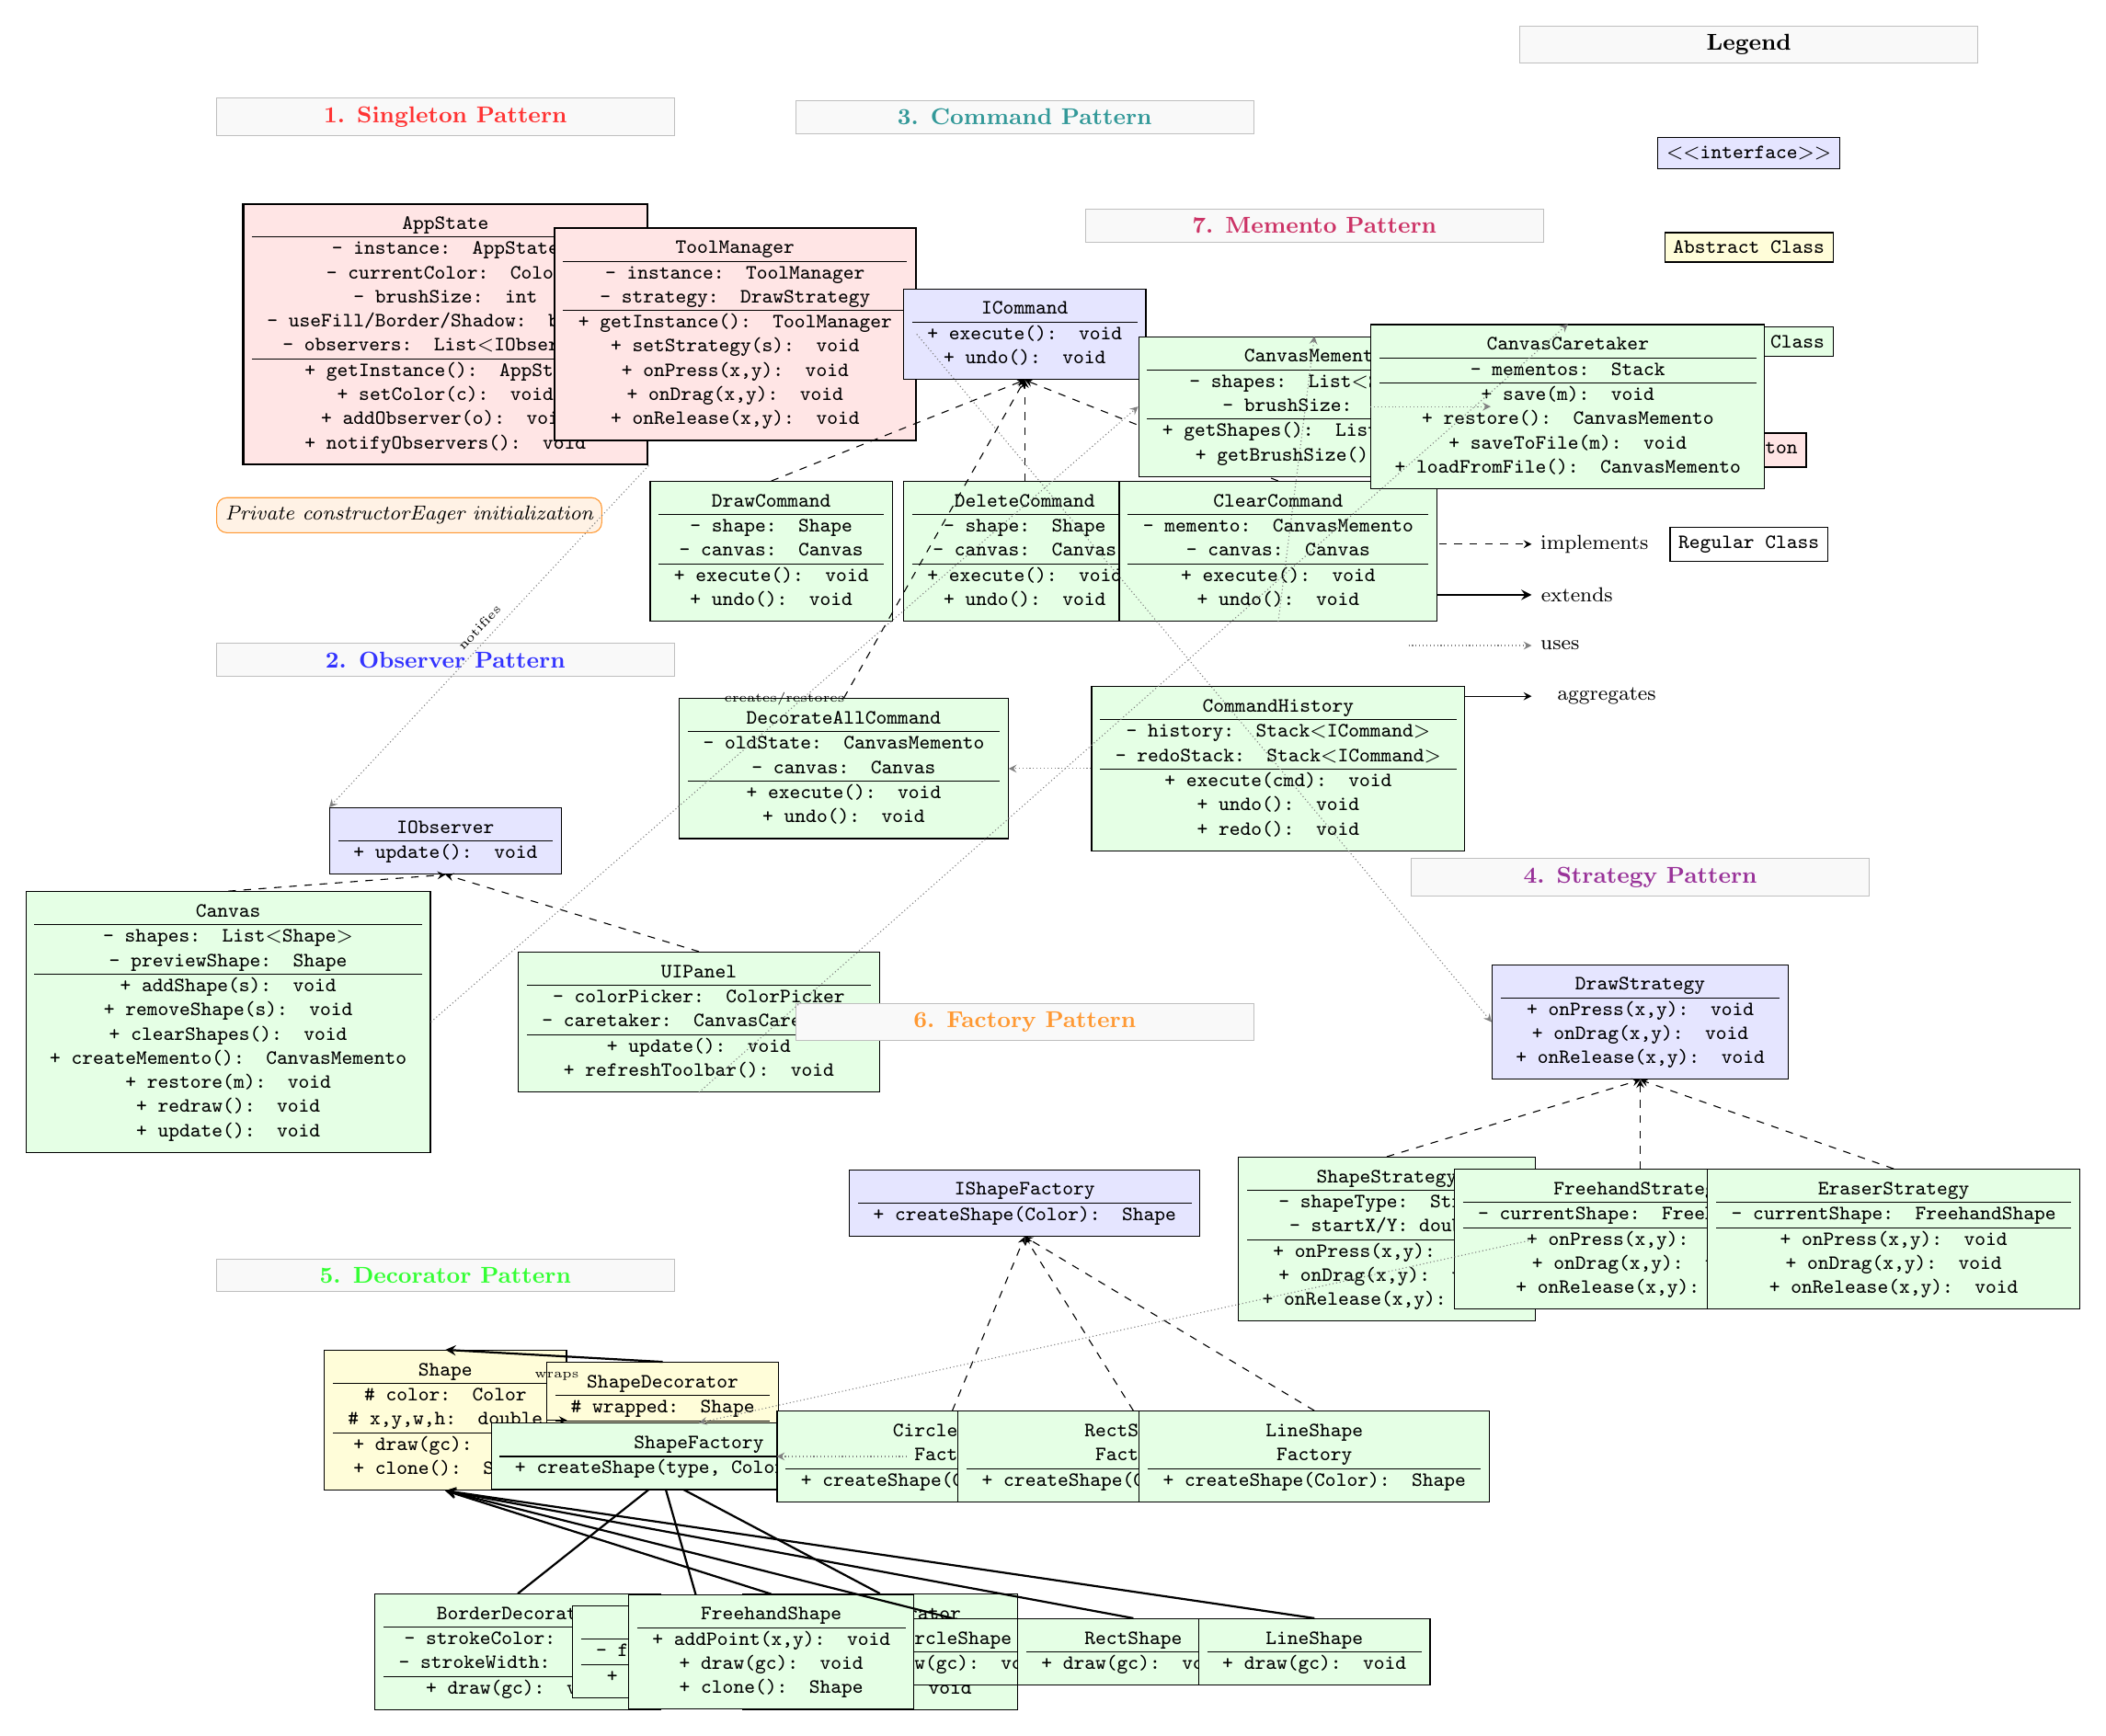
\begin{tikzpicture}
% STYLES
\tikzstyle{interface}=[rectangle, draw=black, fill=blue!10, text centered, font=\footnotesize\ttfamily]
\tikzstyle{abstract}=[rectangle, draw=black, fill=yellow!15, text centered, font=\footnotesize\ttfamily]
\tikzstyle{concrete}=[rectangle, draw=black, fill=green!10, text centered, font=\footnotesize\ttfamily]
\tikzstyle{singleton}=[rectangle, draw=black, fill=red!10, text centered, font=\footnotesize\ttfamily, thick]
\tikzstyle{classstyle}=[rectangle, draw=black, fill=white, text centered, font=\footnotesize\ttfamily]
\tikzstyle{implements}=[->, dashed, >=stealth]
\tikzstyle{extends}=[->, draw=black, thick, >=stealth]
\tikzstyle{uses}=[->, draw=black!50, densely dotted, >=stealth]
\tikzstyle{aggregates}=[->, draw=black, diamond, >=stealth]
\tikzstyle{pattern}=[rectangle, draw=gray!50, fill=gray!5, minimum width=18em, font=\small\bfseries]

% ========================================
% LEGEND
% ========================================
\node[pattern] at (19, 22) {Legend};
\node[interface] at (19, 20.5) {\textless{}\textless{}interface\textgreater{}\textgreater{}};
\node[abstract] at (19, 19.2) {Abstract Class};
\node[concrete] at (19, 17.9) {Concrete Class};
\node[singleton] at (19, 16.4) {Singleton};
\node[classstyle] at (19, 15.1) {Regular Class};

\draw[implements] (14.3,15.1) -- (16,15.1) node[right, font=\footnotesize] {implements};
\draw[extends] (14.3,14.4) -- (16,14.4) node[right, font=\footnotesize] {extends};
\draw[uses] (14.3,13.7) -- (16,13.7) node[right, font=\footnotesize] {uses};
\draw[aggregates] (14.3,13.0) -- (16,13.0) node[right, font=\footnotesize] {aggregates};

% ========================================
% 1. SINGLETON
% ========================================
\node[pattern, text=red!80] at (1, 21) {1. Singleton Pattern};

\node[singleton] (appstate) at (1, 18) {
  \begin{tabular}{c}
    \textbf{AppState}\\
    \hline
    - instance: AppState\\
    - currentColor: Color\\
    - brushSize: int\\
    - useFill\slash Border\slash Shadow: boolean\\
    - observers: List\textless{}IObserver\textgreater{}\\
    \hline
    + getInstance(): AppState\\
    + setColor(c): void\\
    + addObserver(o): void\\
    + notifyObservers(): void\\
  \end{tabular}
};

\node[singleton] (toolmanager) at (5, 18) {
  \begin{tabular}{c}
    \textbf{ToolManager}\\
    \hline
    - instance: ToolManager\\
    - strategy: DrawStrategy\\
    \hline
    + getInstance(): ToolManager\\
    + setStrategy(s): void\\
    + onPress(x,y): void\\
    + onDrag(x,y): void\\
    + onRelease(x,y): void\\
  \end{tabular}
};

\node[rectangle, draw=orange!80, fill=orange!10, font=\footnotesize\itshape, rounded corners] at (0.5, 15.5) {Private constructor\\Eager initialization};

% ========================================
% 2. OBSERVER
% ========================================
\node[pattern, text=blue!80] at (1, 13.5) {2. Observer Pattern};

\node[interface] (iobserver) at (1, 11) {
  \begin{tabular}{c}
    \textbf{IObserver}\\
    \hline
    + update(): void\\
  \end{tabular}
};

\node[concrete] (canvas) at (-2, 8.5) {
  \begin{tabular}{c}
    \textbf{Canvas}\\
    \hline
    - shapes: List\textless{}Shape\textgreater{}\\
    - previewShape: Shape\\
    \hline
    + addShape(s): void\\
    + removeShape(s): void\\
    + clearShapes(): void\\
    + createMemento(): CanvasMemento\\
    + restore(m): void\\
    + redraw(): void\\
    + update(): void\\
  \end{tabular}
};

\node[concrete] (uipanel) at (4.5, 8.5) {
  \begin{tabular}{c}
    \textbf{UIPanel}\\
    \hline
    - colorPicker: ColorPicker\\
    - caretaker: CanvasCaretaker\\
    \hline
    + update(): void\\
    + refreshToolbar(): void\\
  \end{tabular}
};

\draw[implements] (canvas.north) -- (iobserver.south);
\draw[implements] (uipanel.north) -- (iobserver.south);
\draw[uses] (appstate.south east) -- (iobserver.north west) node[midway, above, sloped, font=\tiny] {notifies};

% ========================================
% 3. COMMAND
% ========================================
\node[pattern, text=teal!80] at (9, 21) {3. Command Pattern};

\node[interface] (icommand) at (9, 18) {
  \begin{tabular}{c}
    \textbf{ICommand}\\
    \hline
    + execute(): void\\
    + undo(): void\\
  \end{tabular}
};

\node[concrete] (drawcmd) at (5.5, 15) {
  \begin{tabular}{c}
    \textbf{DrawCommand}\\
    \hline
    - shape: Shape\\
    - canvas: Canvas\\
    \hline
    + execute(): void\\
    + undo(): void\\
  \end{tabular}
};

\node[concrete] (delcmd) at (9, 15) {
  \begin{tabular}{c}
    \textbf{DeleteCommand}\\
    \hline
    - shape: Shape\\
    - canvas: Canvas\\
    \hline
    + execute(): void\\
    + undo(): void\\
  \end{tabular}
};

\node[concrete] (clearcmd) at (12.5, 15) {
  \begin{tabular}{c}
    \textbf{ClearCommand}\\
    \hline
    - memento: CanvasMemento\\
    - canvas: Canvas\\
    \hline
    + execute(): void\\
    + undo(): void\\
  \end{tabular}
};

\node[concrete] (decorateall) at (6.5, 12) {
  \begin{tabular}{c}
    \textbf{DecorateAllCommand}\\
    \hline
    - oldState: CanvasMemento\\
    - canvas: Canvas\\
    \hline
    + execute(): void\\
    + undo(): void\\
  \end{tabular}
};

\node[concrete] (cmdhist) at (12.5, 12) {
  \begin{tabular}{c}
    \textbf{CommandHistory}\\
    \hline
    - history: Stack\textless{}ICommand\textgreater{}\\
    - redoStack: Stack\textless{}ICommand\textgreater{}\\
    \hline
    + execute(cmd): void\\
    + undo(): void\\
    + redo(): void\\
  \end{tabular}
};

\draw[implements] (drawcmd.north) -- (icommand.south);
\draw[implements] (delcmd.north) -- (icommand.south);
\draw[implements] (clearcmd.north) -- (icommand.south);
\draw[implements] (decorateall.north) -- (icommand.south);
\draw[uses] (cmdhist.west) -- (decorateall.east);

% ========================================
% 4. STRATEGY
% ========================================
\node[pattern, text=violet!80] at (17.5, 10.5) {4. Strategy Pattern};

\node[interface] (drawstrategy) at (17.5, 8.5) {
  \begin{tabular}{c}
    \textbf{DrawStrategy}\\
    \hline
    + onPress(x,y): void\\
    + onDrag(x,y): void\\
    + onRelease(x,y): void\\
  \end{tabular}
};

\node[concrete] (shapestrategy) at (14, 5.5) {
  \begin{tabular}{c}
    \textbf{ShapeStrategy}\\
    \hline
    - shapeType: String\\
    - startX\slash Y: double\\
    \hline
    + onPress(x,y): void\\
    + onDrag(x,y): void\\
    + onRelease(x,y): void\\
  \end{tabular}
};

\node[concrete] (freehandstrat) at (17.5, 5.5) {
  \begin{tabular}{c}
    \textbf{FreehandStrategy}\\
    \hline
    - currentShape: FreehandShape\\
    \hline
    + onPress(x,y): void\\
    + onDrag(x,y): void\\
    + onRelease(x,y): void\\
  \end{tabular}
};

\node[concrete] (eraserstrat) at (21, 5.5) {
  \begin{tabular}{c}
    \textbf{EraserStrategy}\\
    \hline
    - currentShape: FreehandShape\\
    \hline
    + onPress(x,y): void\\
    + onDrag(x,y): void\\
    + onRelease(x,y): void\\
  \end{tabular}
};

\draw[implements] (shapestrategy.north) -- (drawstrategy.south);
\draw[implements] (freehandstrat.north) -- (drawstrategy.south);
\draw[implements] (eraserstrat.north) -- (drawstrategy.south);
\draw[uses] (toolmanager.east) -- (drawstrategy.west);

% ========================================
% 5. DECORATOR
% ========================================
\node[pattern, text=green!80] at (1, 5) {5. Decorator Pattern};

\node[abstract] (shape) at (1, 3) {
  \begin{tabular}{c}
    \textbf{Shape}\\
    \hline
    \# color: Color\\
    \# x,y,w,h: double\\
    \hline
    + draw(gc): void\\
    + clone(): Shape\\
  \end{tabular}
};

\node[abstract] (shapedecorator) at (4, 3) {
  \begin{tabular}{c}
    \textbf{ShapeDecorator}\\
    \hline
    \# wrapped: Shape\\
    \hline
    + draw(gc): void\\
    + clone(): Shape\\
  \end{tabular}
};

\node[concrete] (border) at (2, -0.2) {
  \begin{tabular}{c}
    \textbf{BorderDecorator}\\
    \hline
    - strokeColor: Color\\
    - strokeWidth: double\\
    \hline
    + draw(gc): void\\
  \end{tabular}
};

\node[concrete] (filldec) at (4.5, -0.2) {
  \begin{tabular}{c}
    \textbf{FillDecorator}\\
    \hline
    - fillColor: Color\\
    \hline
    + draw(gc): void\\
  \end{tabular}
};

\node[concrete] (shadowdec) at (7, -0.2) {
  \begin{tabular}{c}
    \textbf{ShadowDecorator}\\
    \hline
    - shadowColor: Color\\
    - offset: int\\
    \hline
    + draw(gc): void\\
  \end{tabular}
};

\draw[extends] (shapedecorator.north) -- (shape.north);
\draw[extends] (border.north) -- (shapedecorator.south);
\draw[extends] (filldec.north) -- (shapedecorator.south);
\draw[extends] (shadowdec.north) -- (shapedecorator.south);
\draw[aggregates] (shapedecorator.west) -- (shape.east) node[midway, above, font=\tiny] {wraps};

% ========================================
% 6. FACTORY
% ========================================
\node[pattern, text=orange!80] at (9, 8.5) {6. Factory Pattern};

\node[interface] (ishapefactory) at (9, 6) {
  \begin{tabular}{c}
    \textbf{IShapeFactory}\\
    \hline
    + createShape(Color): Shape\\
  \end{tabular}
};

\node[concrete] (shapefactory) at (4.5, 2.5) {
  \begin{tabular}{c}
    \textbf{ShapeFactory}\\
    \hline
    + createShape(type, Color): Shape\\
  \end{tabular}
};

\node[concrete] (circfactory) at (8, 2.5) {
  \begin{tabular}{c}
    \textbf{CircleShape}\\\textbf{Factory}\\
    \hline
    + createShape(Color): Shape\\
  \end{tabular}
};

\node[concrete] (rectfactory) at (10.5, 2.5) {
  \begin{tabular}{c}
    \textbf{RectShape}\\\textbf{Factory}\\
    \hline
    + createShape(Color): Shape\\
  \end{tabular}
};

\node[concrete] (linefactory) at (13, 2.5) {
  \begin{tabular}{c}
    \textbf{LineShape}\\\textbf{Factory}\\
    \hline
    + createShape(Color): Shape\\
  \end{tabular}
};

\draw[implements] (circfactory.north) -- (ishapefactory.south);
\draw[implements] (rectfactory.north) -- (ishapefactory.south);
\draw[implements] (linefactory.north) -- (ishapefactory.south);

% Concrete shapes
\node[concrete] (circleshape) at (8, -0.2) {
  \begin{tabular}{c}
    \textbf{CircleShape}\\
    \hline
    + draw(gc): void\\
  \end{tabular}
};

\node[concrete] (rectshape) at (10.5, -0.2) {
  \begin{tabular}{c}
    \textbf{RectShape}\\
    \hline
    + draw(gc): void\\
  \end{tabular}
};

\node[concrete] (lineshape) at (13, -0.2) {
  \begin{tabular}{c}
    \textbf{LineShape}\\
    \hline
    + draw(gc): void\\
  \end{tabular}
};

\node[concrete] (freehandshape) at (5.5, -0.2) {
  \begin{tabular}{c}
    \textbf{FreehandShape}\\
    \hline
    + addPoint(x,y): void\\
    + draw(gc): void\\
    + clone(): Shape\\
  \end{tabular}
};

\draw[extends] (circleshape.north) -- (shape.south);
\draw[extends] (rectshape.north) -- (shape.south);
\draw[extends] (lineshape.north) -- (shape.south);
\draw[extends] (freehandshape.north) -- (shape.south);
\draw[uses] (shapefactory.east) -- (circfactory.west);
\draw[uses] (shapestrategy.east) -- (shapefactory.north);

% ========================================
% 7. MEMENTO
% ========================================
\node[pattern, text=purple!80] at (13, 19.5) {7. Memento Pattern};

\node[concrete] (memento) at (13, 17) {
  \begin{tabular}{c}
    \textbf{CanvasMemento}\\
    \hline
    - shapes: List\textless{}Shape\textgreater{}\\
    - brushSize: int\\
    \hline
    + getShapes(): List\textless{}Shape\textgreater{}\\
    + getBrushSize(): int\\
  \end{tabular}
};

\node[concrete] (caretaker) at (16.5, 17) {
  \begin{tabular}{c}
    \textbf{CanvasCaretaker}\\
    \hline
    - mementos: Stack\\
    \hline
    + save(m): void\\
    + restore(): CanvasMemento\\
    + saveToFile(m): void\\
    + loadFromFile(): CanvasMemento\\
  \end{tabular}
};

\draw[uses] (canvas.east) -- (memento.west) node[midway, above, font=\tiny] {creates\slash restores};
\draw[uses] (caretaker.west) -- (memento.east);
\draw[uses] (clearcmd.south) -- (memento.north);
\draw[uses] (uipanel.south) -- (caretaker.north);

\end{tikzpicture}
\end{document}
